\chapter{Arhitektura i dizajn sustava}

	Arhitekturu web aplikacije dijelimo na tri podsustava:
	\begin{itemize}
	\item Web aplikacija
	\item Web poslužitelj
	\item Baza podataka
	\end{itemize}

	%slika arhitekture
	\begin{figure}[H]
		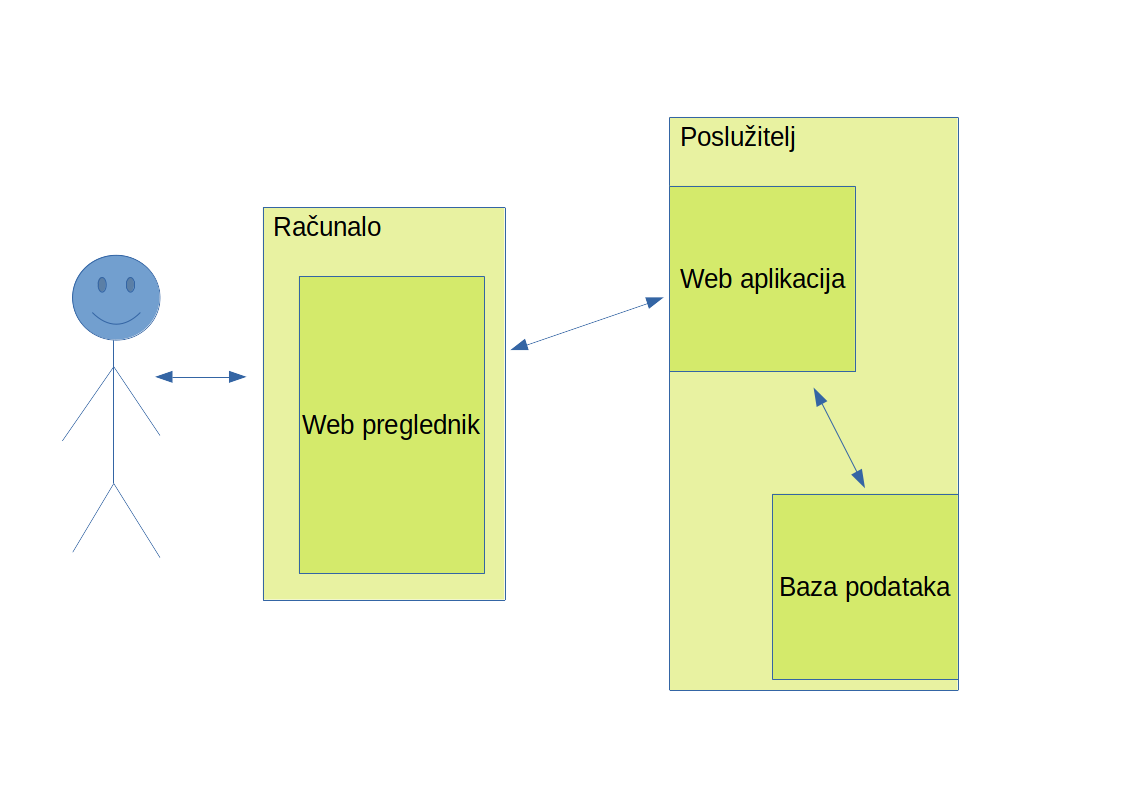
\includegraphics[width=\textwidth]{slike/arhitektura.png}
		\centering
		\caption{Arhitektura sustava}
		\label{fig:arhitektura_sustava}
	\end{figure}
	
	\underline{\textit{Web preglednik}} (eng. \textit{web browser}) je korisnički program koji omogućuje pregledavanje statičkih i dinamičkih sadržaja interneta. Web preglednik dohvaća sadržaj s lokalnog ili udaljenog računala, i potom taj sadržaj interpretira i prikazuje korisniku. Neki od popularnijih web preglednika današnjice su Chrome, Safari, Firefox i Edge.
	
	\underline{\textit{Web poslužitelj}} (eng. \textit{web server}) je temelj aplikacije, a služi za komunikaciju. Korisnik i aplikacija razmjenjuju HTTP zahtjeve (eng. \textit{HTTP request}) i HTTP odgovore (eng. \textit{HTTP response}). Poslužitelj pokreće prednji kraj (eng. \textit{front end}) i stražnji kraj (eng. \textit{back end}). Radi jednostavnosti, baza podataka je također smještena na poslužitelju.
	
	Korisnik kroz grafičko sučelje, odnosno prednji kraj, šalje zahtjeve na REST pristupne točke stražnjeg kraja. Tada stražnji kraj procesuira zahtjev i ako je potrebno komunicira s bazom podataka. Nakon konstrukcije, stražnji kraj šalje odgovor prednjem kraju u obliku JSON objekta, a prednji kraj procesuira odgovor i promjene prikazuje korisniku u obliku HTML stranice. 
	
	Za aplikaciju je odabrana višeslojna arhitektura temeljena na \textbf{MVC} (\textit{model-view-controller}) arhitekturnom stilu te uslužnoj arhitekturi. Podjelu slojeva možemo napraviti na idući način:
	\begin{figure}[H]
		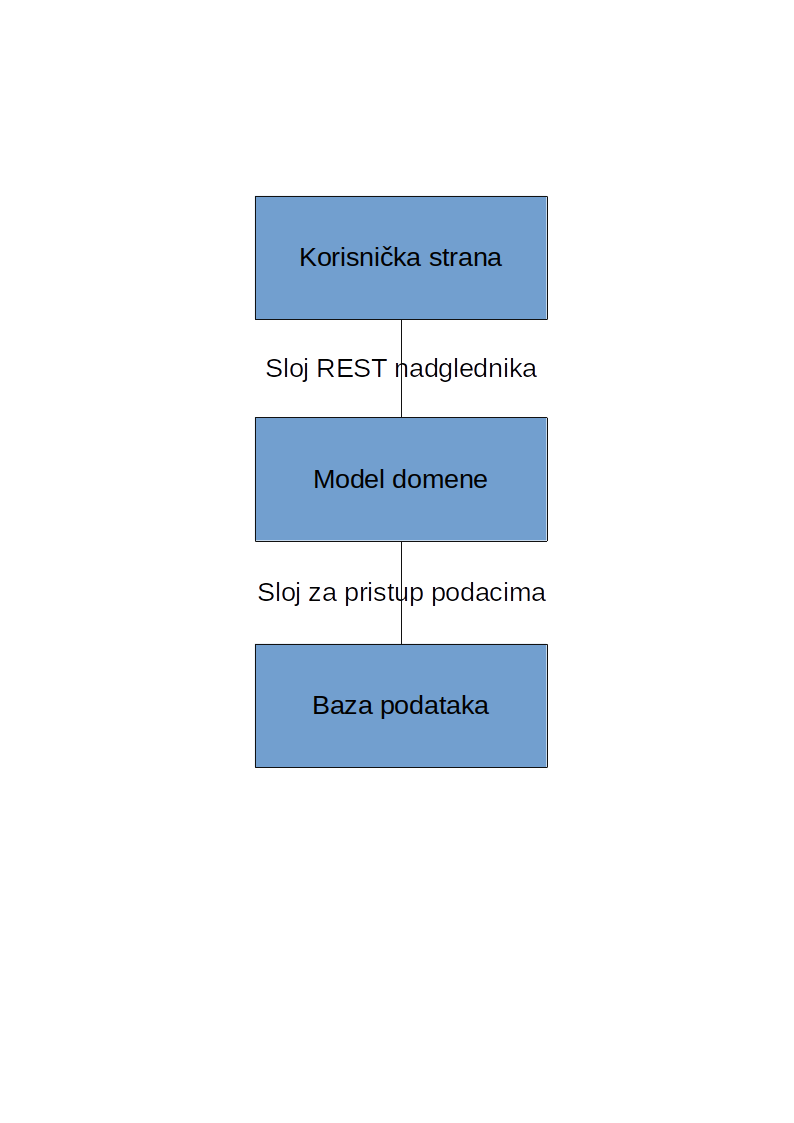
\includegraphics[scale=0.3]{slike/slojevita_arhitektura.png}
		\centering
		\caption{Podjela slojeva}
		\label{fig:podjela_slojeva}
	\end{figure}
	\begin{enumerate}
		\item \textit{sloj korisničke strane} - korisničko sučelje implementirano u JavaScriptu i radnom okviru AngularJS
		\item \textit{sloj nadglednika} - REST nadglednici 
		\item \textit{sloj domene} - model podataka iz domene primjene
		\item \textit{sloj za pristup podacima} - posrednik između sloja domene i baze podataka
		\item \textit{sloj baze podataka} - pohrana podataka
	\end{enumerate}
	
	Ovakva arhitektura odabrana je zbog poželjnih svojstava MVC arhitekturnog stila i višeslojne arhitekture: razvoj pojedinih slojeva jednostavniji je i u velikom stupnju nezavisan od razvoja drugih slojeva. Također, komunikacija prednjeg i stražnjeg kraja je ostvarena primjenom REST arhitketurnog stila. Zbog toga su prednji i stražnji kraj neovisni u smislu jezika implementacije, što potiće ponovnu uporabu.
	
	MVC arhitekturni stil sastoji se od tri koncepta:
	\begin{itemize}
		\item \textbf{Model} - reprezentacija strukture podataka koja se koristi u rješenju, neovisna o korisničkom sučeju
		\item \textbf{View} - pogled na podatke, u našoj aplikaciji to je grafičko sučelje
		\item \textbf{Controller} - nadzornik koji koordinira zahtjeve i odgovore između modela i pogleda, sadrži svu logiku upravljanja.
	\end{itemize}

	REST (\textit{representational state transfer}) arhitekturni stil kao upite koristi URI-je koji su mu poslani i tip HTTP zahtjeva, a odgovara JSON objektom. Tip HTTP zahtjeva koristi se za dohvat, ažuriranje ili umetanje podataka u bazu podataka, a dijelovi URI-ja se koriste za specificiranje zahtjeva. Tako bi na primjer REST API na GET upit usmjeren na putanju /employees odgovorio nizom koji sadrži sve zaposlenike, a GET upit na putanju /employees/user27 bi dobio odgovor JSON objekt koji predstavlja zaposlenika s korisničkim imenom user27.
	
		

				
		\section{Baza podataka}
			
		Odabrali smo PostgreSQL relacijsku bazu podataka za našu web aplikaciju zbog široke korisničke podrške, dokazane stabilnosti, dostupnosti sučelja s Javom, te prijašnjeg iskustva u radu s njom. Relacijska baza podataka omogućuje jednostavno modeliranje problema domene, a temeljna joj je zadaća sigurna i brza pohrana i dohvaćanje podataka. Temeljna građevna jedinica baze podataka je relacija (tablica). Jedna relacija predstavlja jedan entitet, a naša baza sastoji se od idućih relacija:
			
		\begin{itemize}
			\item employees
			\item projects
			\item tasks
			\item teams
			\item workgroups
		\end{itemize}
		
			\subsection{Opis tablica}
			
				\textbf{employees} - Ovaj entitet predstavlja zaposlenika. Sadrži atribute ID, korisničko ime, ime, prezime, lozinka, email, broj telefona, funkciju u firmi te ID tima kojemu pripada. U vezi je \textit{One-to-Many} s entitetom tasks preko atributa ID i u vezi \textit{Many-to-One} s entitetom teams preko atributa ID.		
				\begin{longtabu} to \textwidth {|X[6, l]|X[6, l]|X[20, l]|}
					
					\hline \multicolumn{3}{|c|}{\textbf{employees}}	 \\[3pt] \hline
					\endfirsthead
					
					\hline 
					\endlastfoot
					
					\textbf{emp\_id} & BIGINT	&  jedinstveni identifikator zaposlenika\\ \hline
					emp\_name & VARCHAR & ime zaposlenika \\ \hline
					emp\_surname & VARCHAR & prezime zaposlenika \\ \hline
					emp\_username & VARCHAR & zaposlenikovo korisničko ime \\ \hline
					emp\_password & VARCHAR & zaposlenikova lozinka \\ \hline
					emp\_email & VARCHAR & zaposlenikov email \\ \hline
					emp\_phone & VARCHAR & zaposlenikov broj telefona \\ \hline
					emp\_clearance & INT & zaposlenikova funkcija - developer, team lead, koordinator ili uprava \\ \hline
					\textit{team\_id}	& BIGINT & identifikacijski broj tima kojemu zaposlenik pripada, (teams.team\_id)\\ \hline 		
				\end{longtabu}
			
			
				\textbf{projects} - Ovaj entitet predstavlja projekt. Sadrži atribute ID, opis, ime, te ID tima koji ga je preuzeo. U vezi je \textit{One-to-One} s entitetom teams preko atributa ID tima koji ga je preuzeo.
				\begin{longtabu} to \textwidth {|X[6, l]|X[6, l]|X[20, l]|}
					
					\hline \multicolumn{3}{|c|}{\textbf{projects}}	 \\[3pt] \hline
					\endfirsthead
					
					\hline 
					\endlastfoot
					
					\textbf{project\_id} & BIGINT	&  jedinstveni identifikator projekta\\ \hline
					project\_desc	& VARCHAR & opis projekta	\\ \hline 
					project\_name & VARCHAR &  ime projekta \\ \hline 
					\textit{team\_team\_id} & BIGINT	&  identifikator tima koji rješava projekt, (teams.team\_id)	\\ \hline 					
				\end{longtabu}
			
				\textbf{tasks} - Ovaj entitet predstavlja zadatak na kanban ploči. Sadrži atribute ID, ime, opis, prioritet, status, ID zaposlenika koji ga je preuzeo, te ID tima kojemu pripada. U vezi je \textit{Many-to-One} s entitetom teams preko atributa ID tima kojemu pripada. U istoj je vezi s entitetom employees preko atributa ID korisnika koji ga je preuzeo.
				\begin{longtabu} to \textwidth {|X[6, l]|X[6, l]|X[20, l]|}
					
					\hline \multicolumn{3}{|c|}{\textbf{tasks}}	 \\[3pt] \hline
					\endfirsthead					
					\hline 
					\endlastfoot
					
					\textbf{task\_id} & INT	& jedinstveni identifikator zadatka	\\ \hline
					task\_deadline	& TIMESTAMP &  rok predaje zadatka 	\\ \hline 
					task\_desc & VARCHAR & opis zadatka \\ \hline 
					task\_name & VARCHAR	& ime zadatka\\ \hline 
					task\_prio & INT & prioritet zadatka \\ \hline
					task\_status & INT & status napretka zadatka\\ \hline 
					\textit{emp\_id}	& BIGINT & identifikator zaposlenika koji rješava zadatak, (employee.emp\_id) \\ \hline 
					\textit{team\_id} & BIGINT & identifikator tima kojemu ovaj zadatak pripada, (teams.team\_id)\\ \hline
					
					
				\end{longtabu}
			
			
				\textbf{teams} - Ovaj entitet predstavlja tim zaposlenika u firmi. Sadrži atribute ID tima te ID radne skupine kojoj tim pripada. U vezi je \textit{Many-to-One} s entitetom workgroups preko atributa ID radne skupine kojoj tim pripada i u vezi \textit{One-to-Many} s entitetom employees preko atributa ID. U istoj vezi je s entitetom tasks preko atributa ID. Također je u vezi \textit{One-to-Many} s entitetom projects preko atributa ID.
				\begin{longtabu} to \textwidth {|X[6, l]|X[6, l]|X[20, l]|}
					
					\hline \multicolumn{3}{|c|}{\textbf{teams}}	 \\[3pt] \hline
					\endfirsthead					
					\hline 
					\endlastfoot
					
					\textbf{team\_id} & BIGINT & jedinstveni identifikator tima	\\ \hline
					\textit{wg\_id}	& BIGINT & identifikator radne skupine kojoj ovaj tim pripada, (workgroups.wg\_id)	\\ \hline 
				\end{longtabu}
			
				\textbf{workgroups} - Ovaj entitet predstavlja radnu skupinu. Radna skupina sastoji se od više timova i ima jednog koordinatora. Sadrži atribute ID radne skupine, te ID koordinatora tima. U vezi je \textit{One-to-One} s entitetom employees preko atributa ID koordinatora tima, te je u vezi \textit{One-To-Many} s entitetom teams preko atributa ID radne skupine.
				\begin{longtabu} to \textwidth {|X[10, l]|X[6, l]|X[20, l]|}
					
					\hline \multicolumn{3}{|c|}{\textbf{workgroups}}	 \\[3pt] \hline
					\endfirsthead
					\hline 
					\endlastfoot
					
					\textbf{wg\_id}		 & BIGINT	&  jedinstveni identifikator radne skupine 	\\ \hline
					\textit{coordinator\_emp\_id} 	& BIGINT & identifikator zaposlenika koji je koordinator ove radne skupine  	\\ \hline 
				\end{longtabu}
			
			
			\subsection{Dijagram baze podataka}
			\begin{figure}[H]
				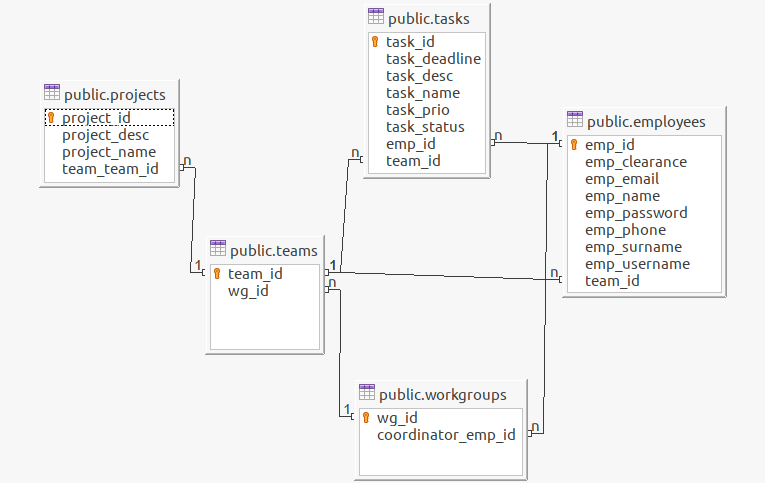
\includegraphics[width=\textwidth]{slike/dijagram_baze.png}
				\centering
				\caption{Dijagram baze podataka}
				\label{fig:dijagram_baze}
			\end{figure}
			
			\eject
			
			
		\section{Dijagram razreda}
		
			Dijagram razreda prikazuje odnose između različitih objekata, te njihove atribute i operacije kojima vladaju. Na slikama 4.3, 4.4 i 4.5 prikazani su razredi koji pripadaju \textit{backend} dijelu naše arhitekture. Radi jednostavnosti, dijagram razreda je podijeljen u više slika, no bez obzira na to, prikazani razredi na neki način komuniciraju.
 			
 			
 			
 			Na idućoj slici prikazan je model podataka kojima backend rukuje. Zaposlenik u firmi modeliran je razredom Employee. Razred Team modelira tim zaposlenika u firmi. Razred Task modelira jedan zadatak na kanban ploči. Razred WorkGroup modelira radnu skupinu u firmi. Razred Project modelira projekt na kojem tim radi.
 			
			\begin{figure}[H]
				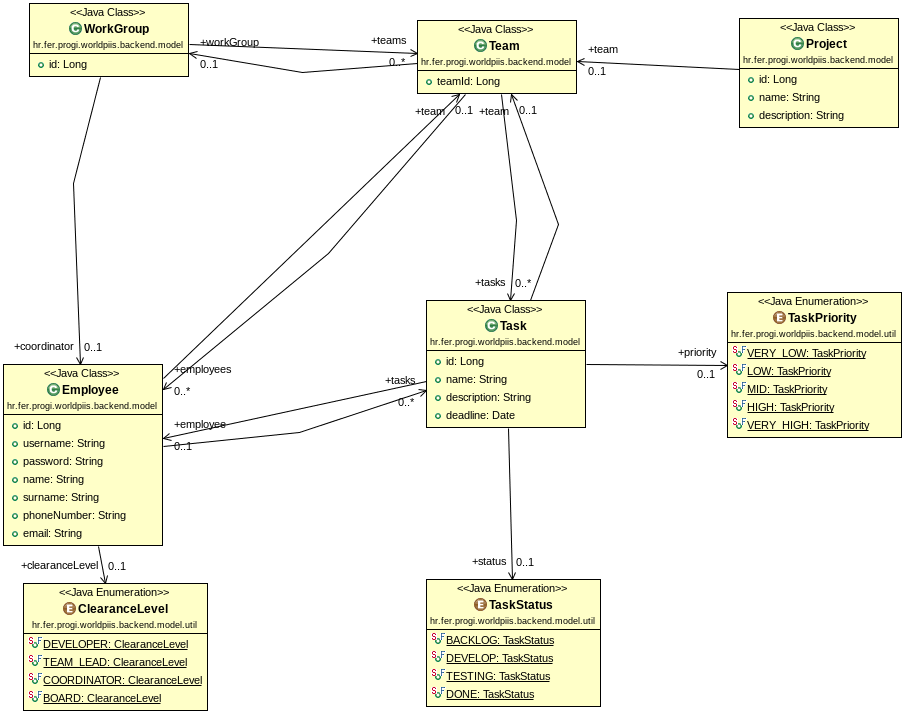
\includegraphics[width=\textwidth]{slike/CLASSD_model.png}
				\centering
				\caption{Dijagram razreda koji opisuje model}
				\label{fig:classd_model}
			\end{figure}
			
			Na idućoj slici prikazana je sredina backenda. Glavni objekt ovdje je sučelje CrudRepository, koje predstavlja apstraktni repozitorij podataka. Iz tog sučelja, izvedena su sučelja ProjectRepository, TaskRepository, TeamRepository, WorkGroupRepository i EmployeeRepository. Ta sučelja predstavljaju repozitorij podataka za prije navedene razrede modela, tj. oni predstavljaju poveznicu s bazom, ili DAO (eng. \textit{Data Access Object}).  
			\begin{figure}[H]
				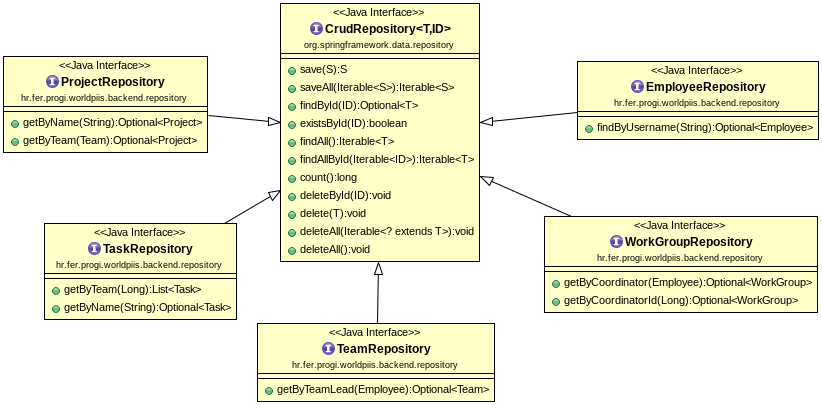
\includegraphics[width=\textwidth]{slike/CLASSD_middle.png}
				\centering
				\caption{Dijagram razreda koji opisuje sredinu backenda}
				\label{fig:classd_middle}
			\end{figure}
		
			Na idućoj slici prikazan je "frontend backenda", odnosno sučelje backenda prema stvarnome svijetu. Ovdje vidimo razrede EmployeeController, TeamController, TaskController, ProjectController i WorkGroupController. Svi ti razredi implementiraju sučelje RestController koje predstavlja REST endpoint. Ti razredi su oni koji dobivaju zahtjeve iz vanjskog svijeta, a odgovaraju HTTP odgovorima i JSON objektima. 
			\begin{figure}[H]
			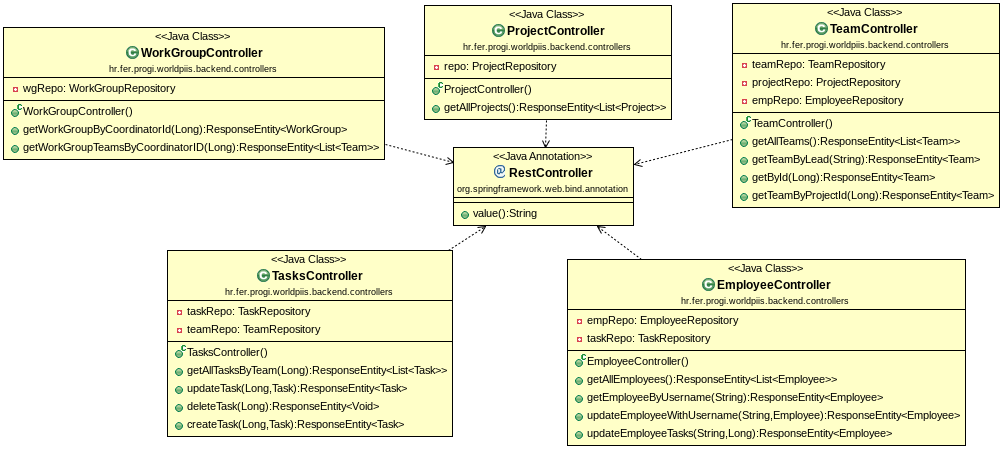
\includegraphics[width=\textwidth]{slike/CLASSD_controllers.png}
			\centering
			\caption{Dijagram razreda koji opisuje prednji dio backenda tj. kontrolere}
			\label{fig:classd_controllers}
			\end{figure}
			\eject
		
		\section{Dijagram stanja}
			
			Dijagram stanja primjenjuje se za opis stanja objekta i za opisivanje prijelaza iz jednog u drugo stanje. Priložena slika prikazuje dijagram stanja objekta "Zadatak". Vođa tima kreira novi zadatak te nakon toga on prelazi u stanje "Backlog". Zadatak u tom stanju preuzima neki razvojni inžinjer ili vođa tima zatim se vraća u to isto stanje. Zaposlenik može započeti razvoj ili testiranje zadataka koji time prelazi u odgovarajuće stanje. Zadatak može ući u stanje "Uređivanje" iz bilo kojeg drugog stanja. U završno stanje dolazi se nakon stanja "Done" što znači da je zadatak izvršen.
			\begin{figure}[H]
				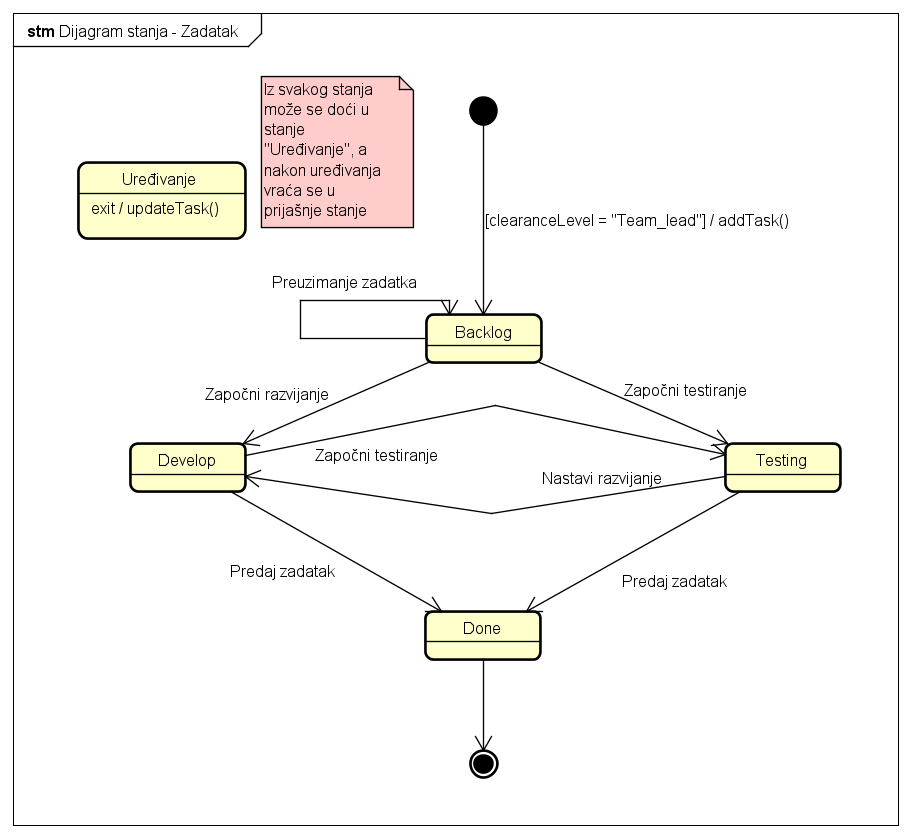
\includegraphics[width=\textwidth]{slike/Dijagram_stanja.png}
				\centering
				\caption{Dijagram stanja}
				\label{fig:classd_middle}
			\end{figure}
			
			
			\eject 
		
		\section{Dijagram aktivnosti}
			
			Dijagram aktivnosti prikazuje povezane aktivnosti na visokoj apstrakcijskoj razini. Dijagram aktivnosti intuitivno prikazuje kako podaci teku kroz aplikaciju i kako se kontrola nad podacima mijenja. Idući dijagram prikazuje proces preuzimanja zadatka i mijenjanja opisa zadatka. Ovaj proces može provesti neki razvojni inženjer ili voditelj tima.
			\begin{figure}[H]
				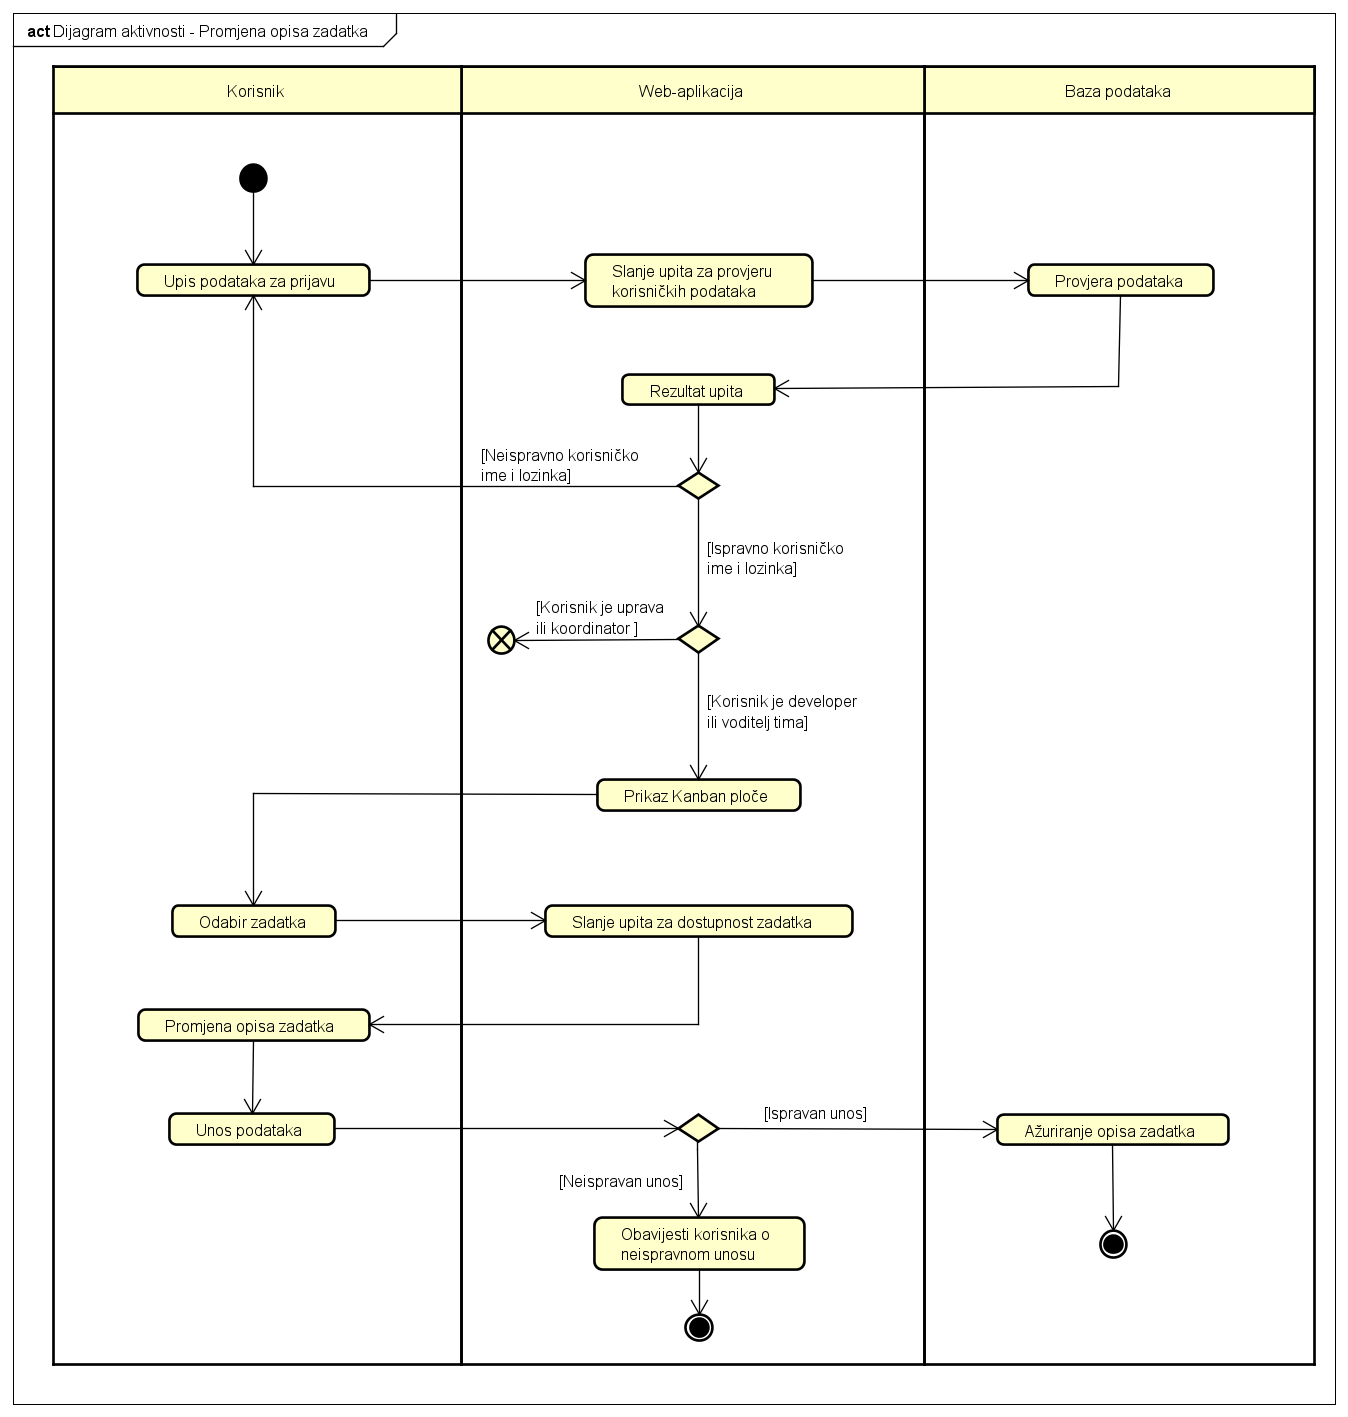
\includegraphics[width=\textwidth]{slike/dijagram_aktivnosti.png}
				\centering
				\caption{Dijagram aktivnosti}
				\label{fig:classd_middle}
			\end{figure}
			
			\eject
		
		\section{Dijagram komponenti}
		
		    Dijagram komponenti omogućuje nam pogled na sustav s visoke razine apstrakcije. Web aplikacija komunicira sa sustavom preko dva sučelja. Prvo sučelje služi za dohvat samih stranica, dakle HTML, CSS i JS datoteka. Drugo sučelje služi za komunikaciju između aplikacije i baze podataka. Dakle, web aplikacija šalje zahtjev REST API-u, koji zauzvrat preko kontrolera komunicira s repozitorijima podataka, koji predstavljaju sloj povezanosti između baze podataka i kontrolera. Repozitoriji dohvaćaju podatke iz baze, preoblikuju ih na način kako je to zapisano u modelima, i prosljeđuju ih kontrolerima. Ovakav način obrade podataka karakterističan je za MVC obrazac. 	
            \begin{figure}[H]
				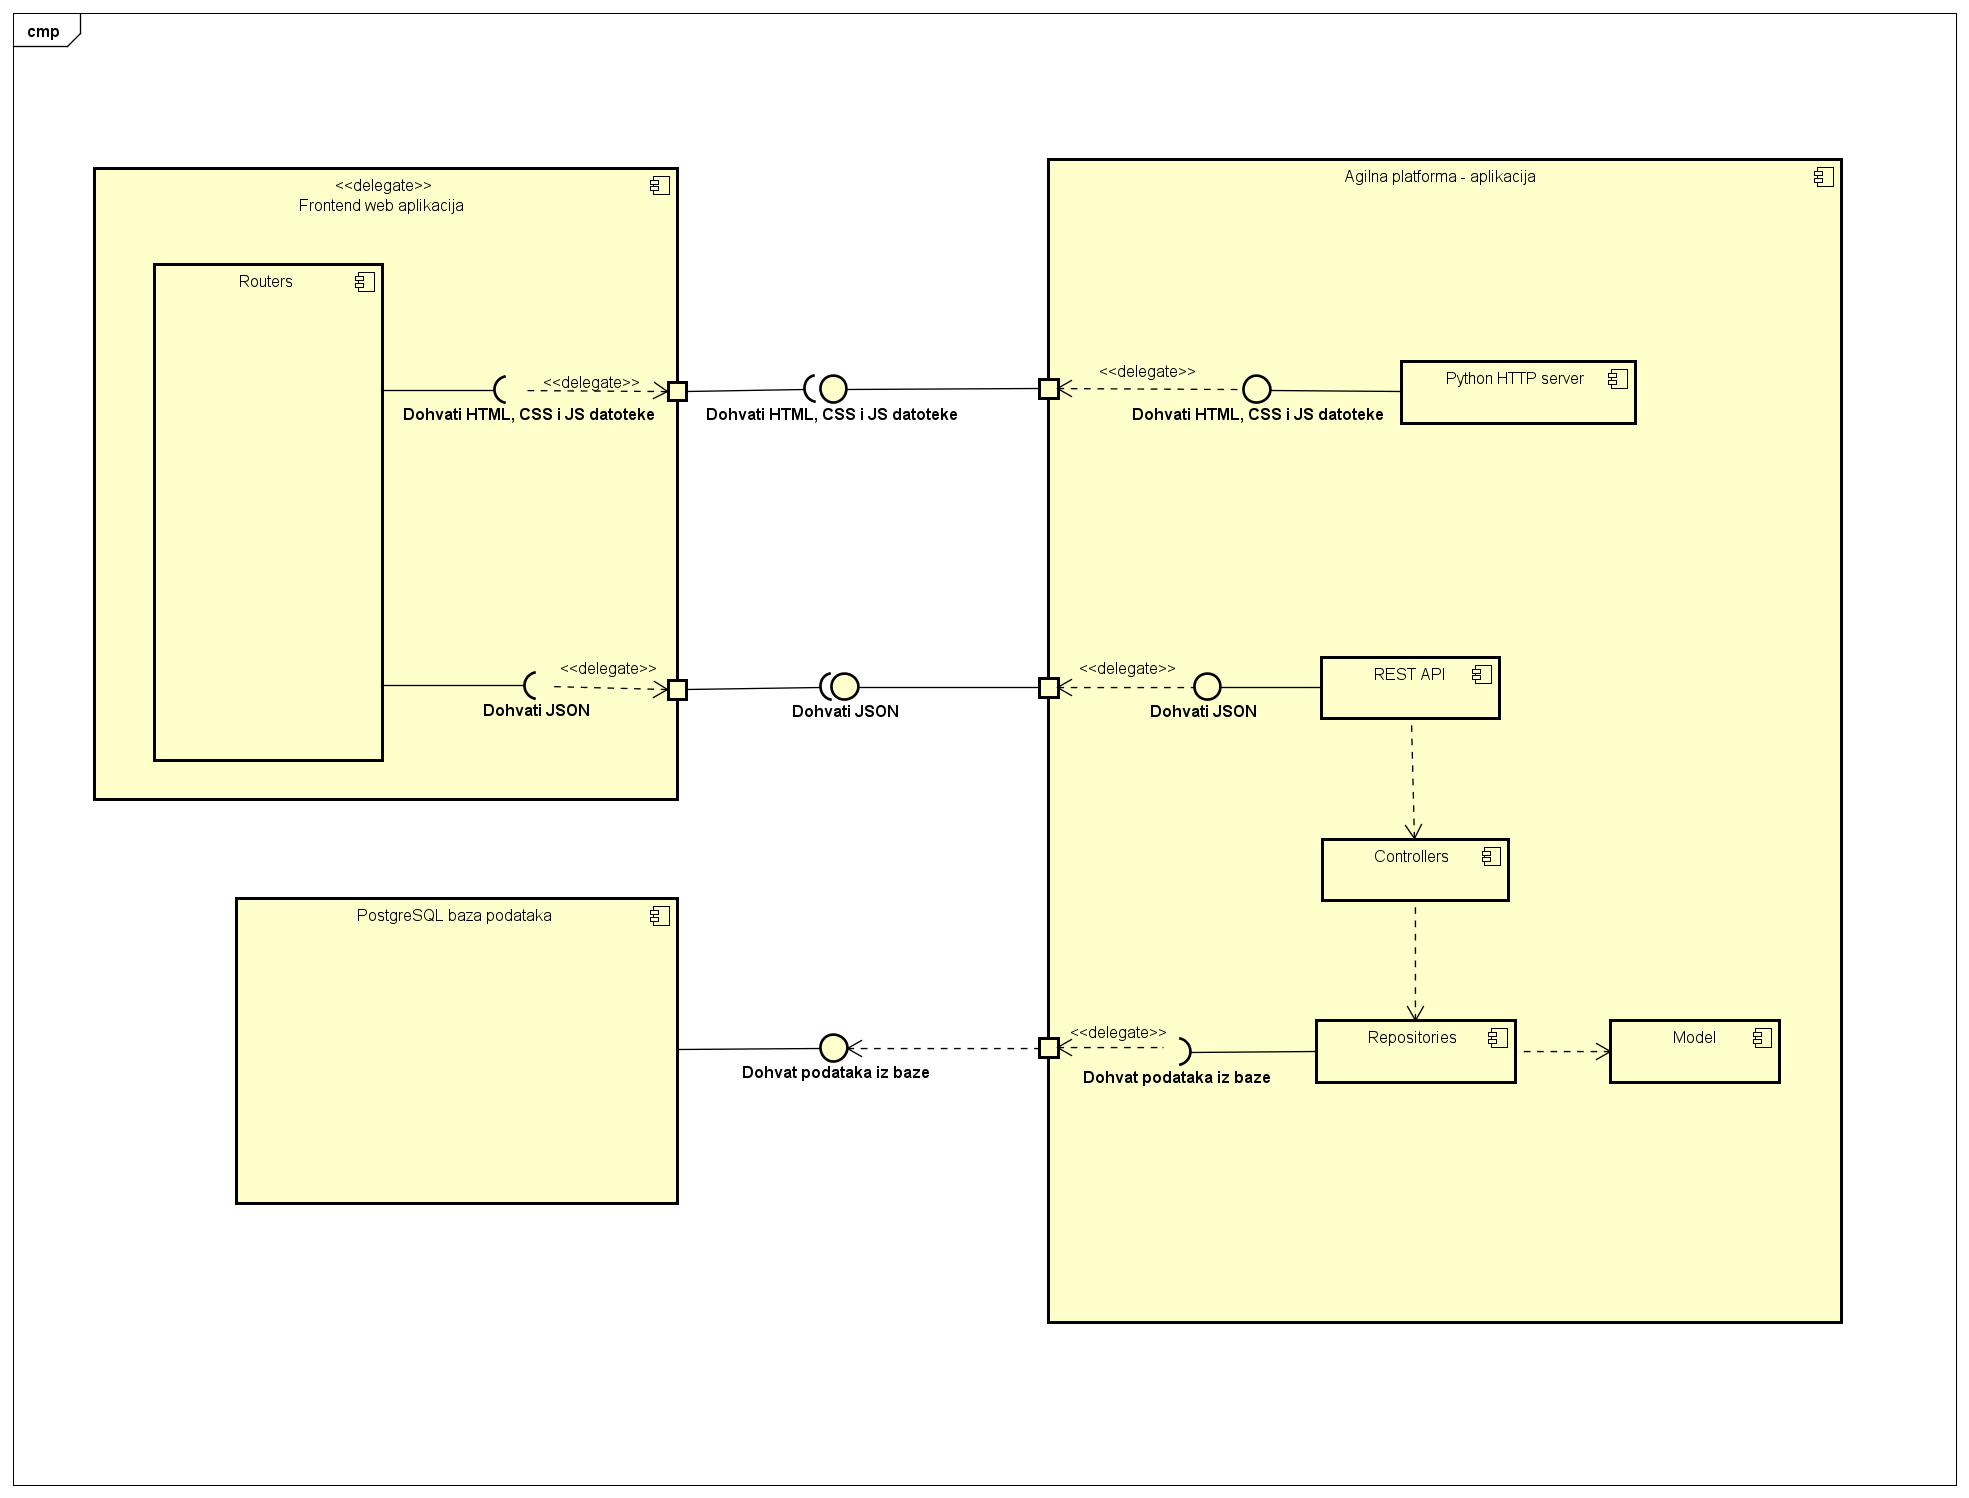
\includegraphics[width=\textwidth]{slike/dijagram_komponenti.png}
				\centering
				\caption{Dijagram komponenti}
				\label{fig:classd_middle}
			\end{figure}
